\chapter{Introduction}\label{ch:introduction}

Placement of the images or paintings on the wall may seem trivial at first.
However, it is not true.
There are different arrangements and constraints to each particular placement.
For example, an art gallery might want to place paintings on the wall, grouping them by their author, style, etc.
One example of such placement can be seen in figure~\ref{fig:london-wall}.
In addition, the room's lighting and the paintings and wall dimensions need to be considered.
Together, these requirements pose a complex problem to solve.

Furthermore, a solution to the painting placement problem can be used in many other, more practical fields.
For example, a facility layout problem (FLP) places a set of facilities on a grid
while having the same constraints as the painting placement – grouping related facilities and considering their dimensions.
Another field is retail shelf-space planning, which tries to partition a shelf into rectangles.
Subsequently, the partitioned shelf is filled with goods that the customers can buy.
Similarly to the lightning conditions for paintings, goods depend on the
particular placement on the shelf – goods close to the customer's eye level increase their visibility and thus lead to more sales.
Last but not least, there is a plethora of packing problems.
One such well-known problem is the 2D rectangular packing problem, which can be reformulated as a knapsack problem.

This thesis proposes a genetic solution to the painting placement problem based on a slicing tree.
It takes a different approach to input parameters and constraints as opposed to some of the
problems mentioned above – inputs are rectangles (paintings) with fixed width and height,
while the same is true for the wall they are placed on. Also, paintings cannot be rotated.
Lastly, there is no constraint on the solution, i.e., the proposed genetic solution can
produce a placement with overlapping paintings or paintings with their parts outside the wall.
A precise definition of the painting placement problem and other mentioned methods can be found in later chapters.

\todo{strucny popis vsech kapitol a struktury prace} Etiam sapien elit, consequat eget, tristique non, venenatis quis, ante. Nemo enim ipsam voluptatem quia voluptas sit aspernatur aut odit aut fugit, sed quia consequuntur magni dolores eos qui ratione voluptatem sequi nesciunt. Suspendisse nisl. Mauris metus. Cras elementum. Etiam ligula pede, sagittis quis, interdum ultricies, scelerisque eu. Fusce suscipit libero eget elit. Cras elementum. Quisque tincidunt scelerisque libero. Maecenas ipsum velit, consectetuer eu lobortis ut, dictum at dui. Cum sociis natoque penatibus et magnis dis parturient montes, nascetur ridiculus mus. Ut tempus purus at lorem. Nulla est. Etiam posuere lacus quis dolor. Maecenas sollicitudin. Mauris tincidunt sem sed arcu. Duis viverra diam non justo. Pellentesque arcu.

\begin{figure}
    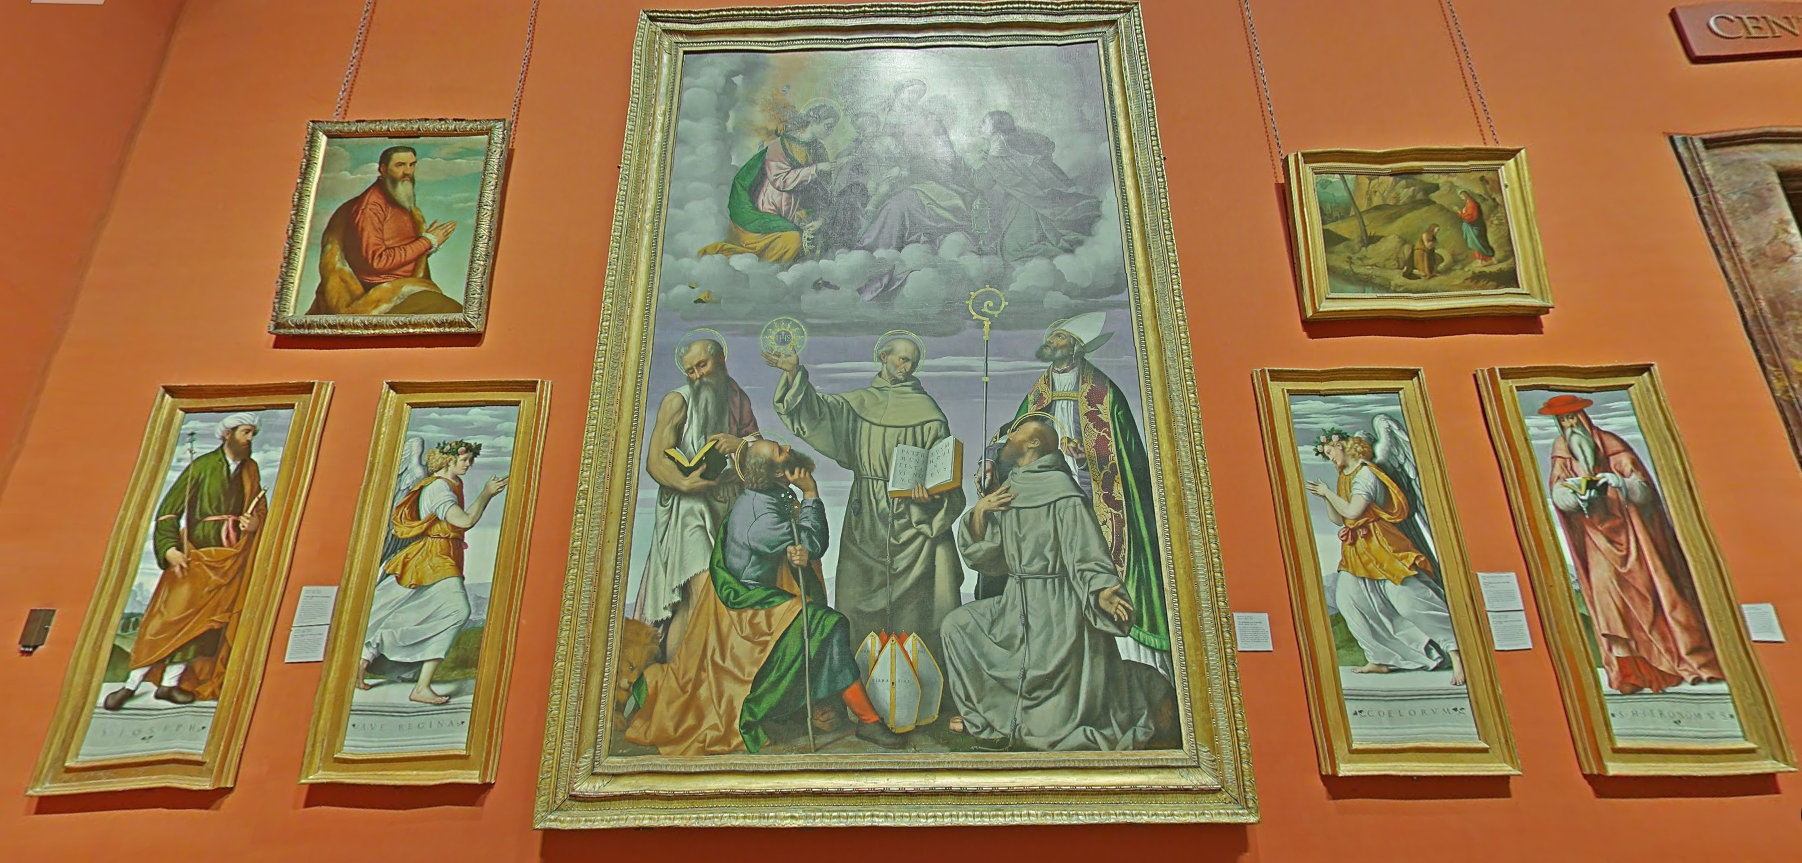
\includegraphics[width=1\textwidth, left]{london_gallery_wall}
    \caption[Painting placement at the London National Gallery]{Painting placement at the London National Gallery. Source~\cite{ScreenshotWallGoogle}:}
    \label{fig:london-wall}
\end{figure}




